\documentclass[xcoler=dvipsnames, aspectratio=169]{beamer}
\usepackage{3191Style}
\newcommand{\abs}[1]{\left|#1\right|}
\date{Brief Markov Chains Introduction}
\begin{document}
    \begin{frame}{Stochastic Matrix}
        \begin{defn}
            \rText{Stochastic Matrix}: We say that a matrix, $A\in\R^{n\times n}$, is a 
            \bText{stochastic matrix} if and only if
            \begin{enumerate}
                \pause\item All elements of $A$ are non-negative. 
                    IE for all $1\leq i,j\leq n$, $a_{ij}\geq 0$
                \pause\item All columns sum to $1$.
            \end{enumerate}
        \end{defn}\pause
        \begin{example}
            \[
                A = \bMat{
                    \frac{1}{2} & \frac{1}{3} & 0\\
                    \frac{1}{2} & \frac{1}{3} & 0\\
                    0 & \frac{1}{3} & 1
                }
            \]
        \end{example}
    \end{frame}
    \begin{frame}{Positive Stochastic Matrix}
        \begin{defn}
            \rText{Positive Stochastic Matrix}: We say that a matrix, $A\in\R^{n\times n}$, is a
            \bText{positive stochastic matrix} if and only if 
            \begin{enumerate}
                \pause\item $A$ is a stochastic matrix
                \pause\item All elements of $A$ are positive.
                    IE for all $1\leq i,j\leq n$, $a_{ij}> 0$
            \end{enumerate}
        \end{defn}\pause
        \begin{example}
            \[
                A = \bMat{
                    .1 & .7 & .3\\
                    .8 & .2 & .3\\
                    .1 & .1 & .4
                }
            \]
        \end{example}
    \end{frame}
    \begin{frame}{Identifying (Positive) Stochastic Matrices}
        Determine which of the following matrices are positive stochastic, stochastic, or neither.\pause
        \[
            A = \bMat{
                .1 & .2 & .7\\
                .2 & .3 & .5\\
                .4 & .5 & .1
            }, B = \bMat{
                .3 & .8 &.15\\
                .3 & .1 &.05\\
                .4 & .1 &.8
            }, C = \bMat{
                .2 & .8 & 0\\
                .7 & .1 &.2\\
                .5 & .1 &.8
            }, D = \bMat{
                .1 & .2 &.2\\
                .3 & .1 &.2\\
                .5 & .1 &.2
            }, E = \bMat{
                .2 & .8 & 0\\
                .3 & .1 &.2\\
                .5 & .1 &.8
            }
        \]
    \end{frame}
    \begin{frame}{Eigenvalues of Stochastic Matrices Part 1}
        \small
        \begin{theorem}
            Let $A\in\R^{n\times n}$ be a stochastic matrix. Then we know that $\lambda=1$ is an
            eigenvalue of $A$ and if $\lambda$ is an eigenvalue of $A$ then $\abs{\lambda}\leq 1$
        \end{theorem}\pause
        \begin{proof}
            First we show that $1$ is an eigenvalue of $A$. Recall that $A$ and $A^\top$ have the 
            same eigenvalues. Since we know that $A$ is stochastic, we know it's columns sum to $1$.
            Therefore, the rows of $A^\top$ also sum to $1$.\pause\ In other words, for each 
            $1\leq i\leq n$
            \[
                \sum_{j=1}^n\left(A^\top\right)_{ij}\pause = 
                \sum_{j=1}^n A_{ji}\pause = 1
            \]
            Let $\vec{1}_n$ be the vector of all $1$'s, then\pause
            \[
                A^\top\vec{1}_n = \vec{1}_n
            \]
            So, $(\lambda,\vec{1}_n)$ is an eigenpair of $A$.
        \end{proof}
    \end{frame}
    \begin{frame}{Eigenvalues of Stochastic Matrices Part 2}
        \footnotesize
        \begin{theorem}
            Let $A\in\R^{n\times n}$ be a stochastic matrix. Then we know that $\lambda=1$ is an
            eigenvalue of $A$ and if $\lambda$ is an eigenvalue of $A$ then $\abs{\lambda}\leq 1$
        \end{theorem}\pause
        \begin{proof}
            Now, we will show that if $\lambda$ is an eigenvalue of $A$, then $\abs{\lambda}\leq 1$.\pause

            Recall as before that $A$ and $A^\top$ share eigenvalues, so let $(\lambda,\vec{x})$
            be an eigenpair of $A^\top$.\pause\ This means $A^\top\vec{x} = \lambda\vec{x}$.\pause\
            Consider the $j^\text{th}$ entry of $\lambda\vec{x}$.
            \vspace{-5pt}
            \[
                (\lambda\vec{x}) = \lambda x_j = \sum_{i=1}^n A_{ij}x_i
            \]\pause\
            If we pick the index $j$ such that $\abs{x_j}\leq\abs{x_i}$ for all $i$, 
            then we have that\pause\
            \[
                \abs{\lambda x_j} = \abs{\lambda}\abs{x_j}\pause = \abs{\sum_{i=1}^n A_{ij}x_i}
                \pause\leq \sum_{i=1}^n\abs{A_{ij}}\abs{x_i}\pause = \sum_{i=1}^nA_{ij}\abs{x_i}
                \pause\leq \sum_{i=1}^nA_{ij}\abs{x_j}\pause = \abs{x_j}\sum_{i=1}^nA_{ij}\pause = 
                \abs{x_j}
            \]\pause\
            Dividing by $\abs{x_j}$ gives us that $\abs{\lambda}\leq 1$
        \end{proof}
    \end{frame}
    \begin{frame}{Eigenvalues of Positive Stochastic Matrices}
        \begin{theorem}
            If $A$ is a positive stochastic matrix, then $\dim{E(A,1)} = 1$.
        \end{theorem}
        \vspace{130pt}
    \end{frame}
    \begin{frame}{A (Very) Simple Weather Model}
        \footnotesize
        We will model weather as follows
        \begin{enumerate}[a)]
            \pause\item There are two states: (1) Sunny and (2) Rainy
            \pause\item The current weather can always be observed
            \pause\item The current weather informs the weather for tomorrow, and we know the probability
                of tomorrow's weather given today's weather
        \end{enumerate}\pause\
        \vspace{10pt}
        \begin{columns}
            \column{.5\textwidth}
            We can build a model to predict the weather. An example is given below\pause\\
            \begin{center}
                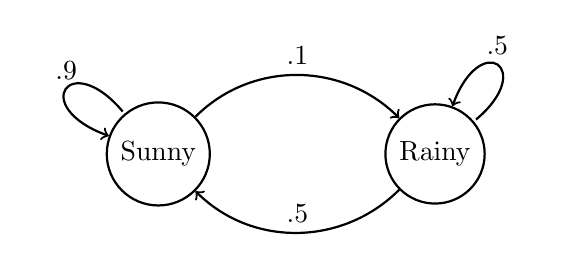
\begin{tikzpicture}[node distance={100pt}, thick, main/.style = {draw, circle}]
                    \node[main] (1) {Sunny};
                    \node[main] (2)[right of=1] {Rainy};
                    \draw[->] (1) to [out=45,in=135] node[midway,above]{.1}(2);
                    \draw[->] (2) to [out=225,in=315] node[midway,above]{.5}(1);
                    \draw[->,shorten <= 1pt] (1) to [out=130,in=160,loop] node[midway,above]{.9}(1);
                    \draw[->,shorten <= 1pt] (2) to [out=40,in=70,loop] node[midway,above]{.5}(2);
                \end{tikzpicture}
            \end{center}
            \column{.5\textwidth}
            \begin{enumerate}
                \pause\item If we assign each node a number from $1$ to $n$ where $n$ is 
                    the number of states we have we can collect these in a transition matrix $P$.\pause\
                    \[
                        P = \bMat{
                            .9 & .5 \\
                            .1 & .5
                        }
                    \]
                    \vspace{-12pt}
                \pause\item $P_{ij}$ is the probability of going from state $i$ to state $j$.
                \pause\item $P$ is also a stochastic matrix!
            \end{enumerate}
        \end{columns}
    \end{frame}
    \begin{frame}{Markov Chains in a Nutshell}
        \begin{tcolorbox}
            An intuitive view of a Markov Chain is a math model describing some kind of ``experiment''
            a large number of times under the same condition
            \only<1>{\vspace{63pt}}
            \only<2->{
                \begin{itemize}
                    \only<2->{\item Each experiment has the same $n$ possible outcomes}
                    \only<2>{\vspace{46pt}}
                    \only<3->{\item There is some set of probabilistic rules that determine how the system moves
                        from one state to another}
                    \only<3>{\vspace{18pt}}
                    \only<4->{\item These probabilities only depend on the current state}
                \end{itemize}
            }
        \end{tcolorbox}
        \only<1-4>{\vspace{12pt}}
        \only<5>{This can be applied to many fields including: Epidemiology, Finance, Statistics, etc.}
    \end{frame}
    \begin{frame}{Markov Chains in Terms of Linear Algebra}
        \begin{tcolorbox}
            A more formal definition with the tools that we have is as follows:

            A \bText{Markov chain} is a sequence of \bText{state vectors}
            $\vec{x}_0,\vec{x}_1,\vec{x}_2,\dots$ in $\R^{n}$ and a 
            
            \bText{stochastic} (transition) \bText{matrix} $P$ such that for $k=0,1,2,\dots$
            \[
                \vec{x}_{k+1} = P\vec{x}_k
            \]
        \end{tcolorbox}\pause
        Where $\vec{x}_k = \bMat{p_1\\\vdots\\p_n}$ is a vector of probabilities we are in each
        state $1,\dots n$.
    \end{frame}
    \begin{frame}{Revisiting our (Very) Simple Weather Model}
        Recall that our simple weather model has transition matrix: $P=\bMat{.9 & .5\\.1 & .5}$.\pause\
        Lets say that it is sunny today, so our initial state vector is $\vec{x}_0 = \bMat{1\\0}$
        and we want to figure out how likely it is to be each kind of weather $3$ days from today.\pause\
        We want to find $\vec{x}_3$.\pause
        \[
            \vec{x}_3 = P\vec{x}_2\pause = P(P\vec{x}_1)\pause = P(P(P\vec{x}_0))\pause = P^3\vec{x}_0
        \]\pause
        We just compute 
        \[
            P^3 = \bMat{
                .844 & .78\\
                .156 & .22
            }
        \]\pause
        So, 
        \[
            \vec{x}_3 = P^3\vec{x}_0\pause = \bMat{
                .844 & .78\\
                .156 & .22
            }\bMat{1\\0}\pause = \bMat{.844\\.156}
        \]
    \end{frame}
    \begin{frame}{Property of Powers of Positive Stochastic Matrices}
        \begin{theorem}
            Let $A\in\R^{n\times n}$ be a diagonalizable positive stochastic matrix. Then, for some
            large $n$, we have that\pause
            \[
                A^n = \left(VDV^{-1}\right)^n\pause = VD^nV^{-1}\pause\approx V\bMat{
                    1 & 0 & \dots & 0\\
                    0 & 0 & \dots & 0\\
                    \vdots & \vdots & \vdots & \vdots\\
                    0 & 0 & \dots & 0\\
                }V^{-1}
            \]
        \end{theorem}\pause
        \emph{Note}: We can say something very similar for non-diagonalizable matrices, but it's
        harder to phrase
    \end{frame}
    \begin{frame}{Steady State (Equilibrium)}
        \begin{defn}
            \rText{Steady State}: The \bText{steady state} of a stochastic matrix $A$ is an eigenvector
            $\vec{v}$ associated with $\lambda=1$ such that all the entries are \emph{positive} and 
            sum to $1$.
        \end{defn}\pause
        This solution is a representation of what happens in the long run of a Markov chain!\pause

        Computing this can be challenging in general if our Eigenspace associated with $\lambda=1$
        has more than one basis vector.
    \end{frame}
    \begin{frame}{Steady State of a Positive Stochastic Matrix}
        However, if $A\in\R^{n\times n}$ is a \emph{positive} stochastic matrix, then we know 
        $\dim{E(A,1)} = 1$.\pause\ Meaning, it's a lot easier! We can just:
        \begin{enumerate}
            \pause\item Solve $(A-I_n)\vec{v}=\vec{0}$
            \pause\item Divide $\vec{v}$ by the sum of its elements.
            \pause\item This new vector is the steady state vector!
        \end{enumerate}
    \end{frame}
    \begin{frame}{Steady State Example}
        Let's find the steady state of a different stochastic matrix
        \[
            P = \bMat{
                .3 & .4 & .5\\
                .3 & .4 & .3\\
                .4 & .2 & .2
            }
        \]
        See Jupyter Notebook
    \end{frame}
    \begin{frame}{A Practical Application: PageRank}
        The original algorithm that Google used in it's search engine was based on PageRank, which 
        ranks websites based on the number of links to and from it.

        \vspace{10pt}

        The textbook discusses it in the end of chapter 5.6: \url{https://textbooks.math.gatech.edu/ila/stochastic-matrices.html}. 

        \vspace{10pt}

        A more comprehensive history can be found at the wikipedia page: \url{https://en.wikipedia.org/wiki/PageRank\#History}
    \end{frame}
\end{document}
